O salto ornamental � um esporte em que cada competidor realiza seis saltos. A nota em cada salto � calculada pela soma das notas dos ju�zes, multiplicada pela nota de partida ( o grau de dificuldade de cada salto). Fica em primeiro lugar o atleta que obtiver a maior soma das seis notas recebidas. 
O atleta 1 O ir� realizar o �ltimo salto da final. Ele observa no Quadro 1, antes de executar o salto, o recorte do quadro parcial de notas com a sua classifica��o e a dos tr�s primeiros lugares at� aquele momento.

\begin{figure}[h]
\centering
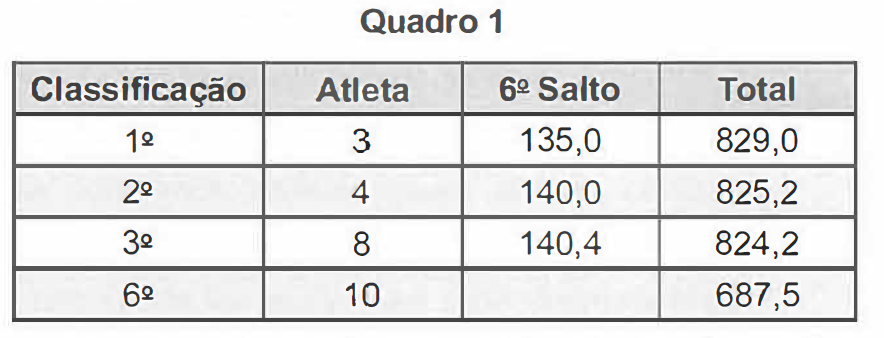
\includegraphics[width=8cm]{../figuras/q161(1)-2018.png}
\end{figure}

Ele precisa decidir com seu treinador qual salto dever� realizar. Os dados dos poss�veis tipos de salto est�o no Quadro 2. 

\begin{figure}[h]
\centering
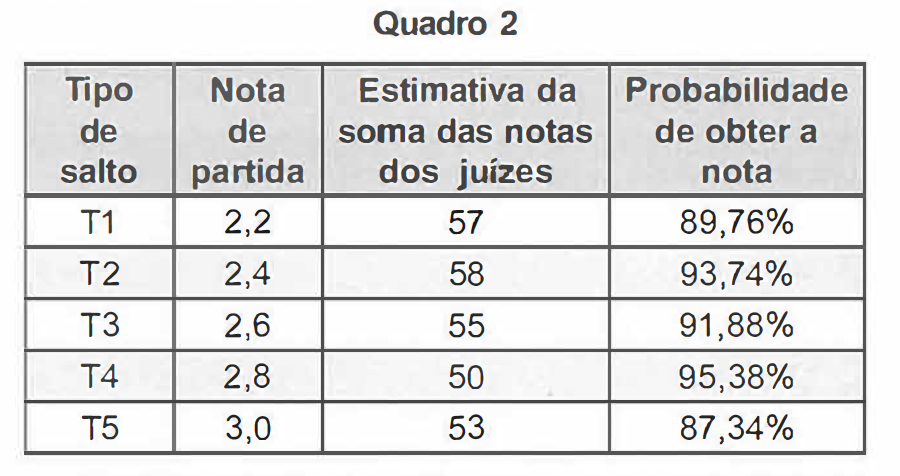
\includegraphics[width=8cm]{../figuras/q161(2)-2018.png}
\end{figure}


O atleta optar� pelo salto com a maior probabilidade de obter a nota estimada, de maneira que lhe permita alcan�ar o primeiro lugar. 
Considerando essas condi��es, o salto que o atleta dever� escolher � o de tipo 

\begin{enumerate}
\item[a)]T1
\item[b)]T2
\item[c)]T3
\item[d)]T4
\item[e)]T5
\end{enumerate}